\documentclass{standalone}
\usepackage{pgfplots}
\usetikzlibrary{decorations.markings}

\definecolor{lightblue}{RGB}{50,97,181}
\definecolor{lightred}{RGB}{232,39,31}

\pgfplotsset{
    ondrej's graphs/.style={
        domain=0.2:4,
        xmin=0,xmax=5,
        ymin=0,
        axis lines=left,
        xtick=\empty, ytick=\empty,
        xlabel=$c_t$,
        ylabel=$c_{t+1}$,
        every axis title/.style={
            align=center, at={(0.5,1.1)},
	  font=\bf
        },
        every axis y label/.style={
            at={(current axis.above origin)},
            anchor=east
        },
        every axis x label/.style={
            at={(current axis.right of origin)},
            anchor=north
        },
        cycle list={
            ultra thick, orange, no markers, smooth,samples=500\\
        },
        shift function/.style 2 args={
            x filter/.code={\pgfmathparse{\pgfmathresult+##1}},
            y filter/.code={\pgfmathparse{\pgfmathresult+##2}}
        },
        /tikz/tangent line/.style={
            ultra thick, black, shorten <=-4cm, shorten >=-4cm,
            insert path={(tangent.west) -- (tangent.east)}
        },
        /tikz/indicator lines/.style={
            thin, densely dashed
        },
        /tikz/point/.style={
            fill=red,
            radius=3pt,
	draw=red!50!black
        },
        project point on axes/.code={
            \pgfplotsset{/pgfplots/after end axis/.code={
                \draw [indicator lines]
                (tangent-|{rel axis cs:0,0}) 
                node [anchor=east] {$c_{t+1}^*$} 
                -| (tangent|-{rel axis cs:0,0})
                node [anchor=north] {$c_t^*$};
	     \draw [point] (tangent) circle;
            }}
        },
        /tikz/label node/.style={
            font=\small,
            align=left,
            anchor=west
        }
    }
}

\tikzset{
        tangent point/.style={
            sloped,
            name=tangent,
            pos=#1
        },
        tangent point/.default=0.5
}

\begin{document}
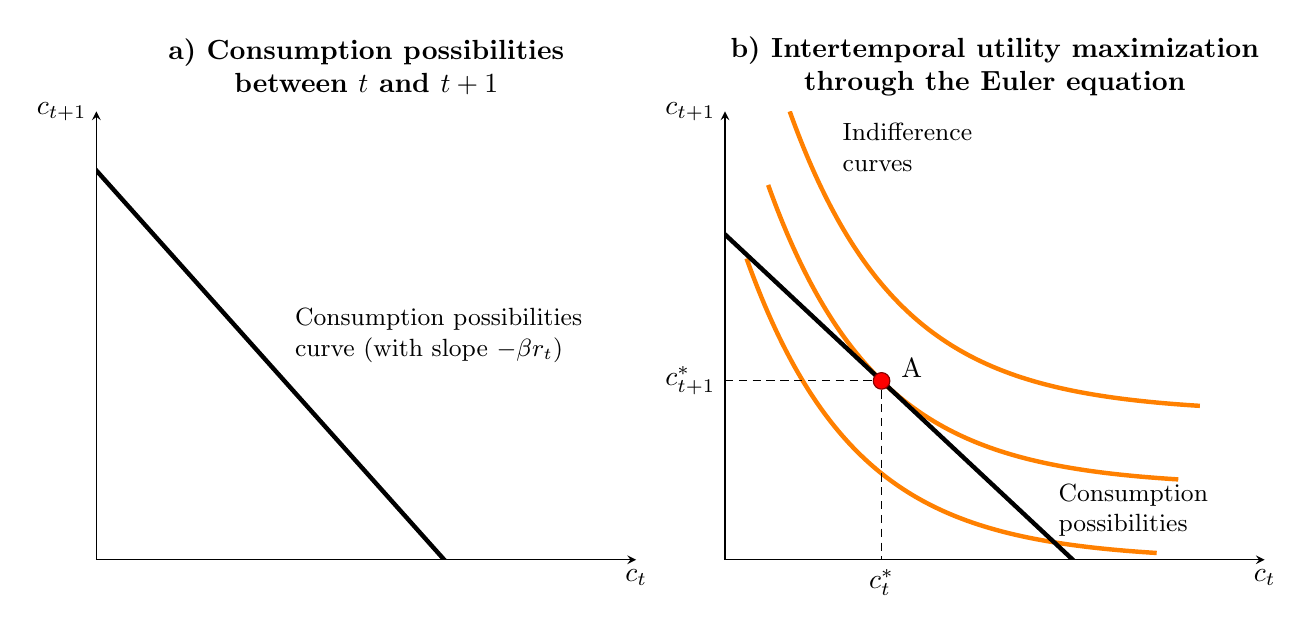
\begin{tikzpicture}



\begin{axis}[ondrej's graphs,name=plot1,
title=a) Consumption possibilities \\between $t$ and $t+1$]
\addplot +[shift function={0.2}{0.2},white] {e^(-x)} node [tangent point=0.3] {};
\draw [tangent line];
\node [label node] at (rel axis cs:0.35,0.5) {Consumption possibilities \\  curve (with slope $-\beta r_{t}$)};
\end{axis}



\begin{axis}[ondrej's graphs,name=plot2,at=(plot1.right of south east), anchor=left of south west,
title=b) Intertemporal utility maximization \\ through the Euler equation]
\addplot {e^(-x)};
\addplot +[shift function={0.2}{0.2}] {e^(-x)} node [tangent point=0.3] {};
\addplot +[shift function={0.4}{0.4}] {e^(-x)};
\draw [tangent line] node [anchor=south west] {A};
\pgfplotsset{project point on axes}
\node [label node] at (rel axis cs:0.2,0.92) {Indifference\\curves};
\node [label node] at (rel axis cs:0.6,0.11) {Consumption \\ possibilities};
\end{axis}


\end{tikzpicture}
\end{document} 